\chapter{Conceptos b\'{a}sicos}

\section{Definici\'{o}n de segmentaci\'{o}n}

La segmentaci\'{o}n de imagen, tambi\'{e}n denominada a veces como \textit{labelling}, es el proceso de dividir la imagen en grupos o regiones contiguas cuyos elementos(p. e. p\'{i}xeles o \textit{voxels}) tienen propiedades o caracter\'{i}sticas comunes. Estas regiones servir\'{a}n para identificar los objetos de la imagen que posteriormente podr\'{a}n ser clasificados y etiquetados en base a sus propiedades \cite{terry1}. 

El resultado final de la segmentaci\'{o}n de la imagen ser\'{a} un conjunto de regiones o segmentos que formar\'{a}n la imagen original. Cada uno de los p\'{i}xeles de una regi\'{o}n tendr\'{a} una caracter\'{i}stica com\'{u}n con los p\'{i}xeles de dicha regi\'{o}n y una diferencia significativa respecto a p\'{i}xeles de otra regi\'{o}n, por ello se habr\'{a}n agrupado en distinto segmento, ya sea por ejemplo, en el color, la textura o la intensidad. Por lo tanto, se podr\'{a}n extraer los segmentos de inter\'{e}s de la imagen, es decir, los objetos que \'{e}sta contiene.

\section{Evoluci\'{o}n de la segmentaci\'{o}n}\label{cap:EvoSeg}

Los primeros desarrollos en el \'{a}mbito de la segmentaci\'{o}n de imagen se remontan a hace 50 a\~{n}os. En 1965 se desarroll\'{o} un operador para detectar bordes entre diferentes partes de una imagen, conocido como \textit{Roberts operator} o \textit{Roberts Edge Detector}. Este detector fue el primer paso hacia la descomposici\'{o}n de im\'{a}genes en diferentes segmentos o regiones. En esa misma d\'{e}cada tambi\'{e}n se propusieron varios detectores de bordes como \textit{Sobel} y \textit{Prewitt edge detectors}. A partir de ah\'{i}, comenzaron a surgir diferentes algoritmos y t\'{e}cnicas de segmentaci\'{o}n. Junto con esto, tambi\'{e}n se ampli\'{o} el \'{a}mbito de estas t\'{e}cnicas: de imagen 2D a 3D, de im\'{a}genes fijas a im\'{a}genes en <<movimiento>> o secuencias de im\'{a}genes, de escalas de gris a im\'{a}genes a color etc \cite{zhang1}.

A pesar de los a\~{n}os de investigaci\'{o}n dedicados a estas t\'{e}cnicas y el gran n\'{u}mero de ellas existentes, la segmentaci\'{o}n de imagen sigue siendo un tema de investigaci\'{o}n desafiante y no existe a\'{u}n un est\'{a}ndar de segmentaci\'{o}n que funcione bien para cualquier tipo de imagen. Estas t\'{e}cnicas est\'{a}n en continua evoluci\'{o}n y a\'{u}n est\'{a}n lejos de su madurez. Prueba de ello est\'{a} en que muchas conferencias del \'{a}mbito de tratamiento de imagen tienen apartados de segmentaci\'{o}n, adem\'{a}s, el n\'{u}mero de art\'{i}culos de este \'{a}mbito aumenta cada a\~{n}o y muchos libros de procesamiento de imagen tienen cap\'{i}tulos referidos a la segmentaci\'{o}n \cite{zhang1}.

Para que el lector se haga una idea, se ha realizado una b\'{u}squeda en el sitio web \textit{ieee explore}\cite{ieee1} con las palabras <<image segmentation>> en varios a\~{n}os. Este buscador encuentra art\'{i}culos, conferencias, est\'{a}ndares, libros, revistas y cursos de aprendizaje relacionados con las palabras introducidas. La figura \ref{regisIEEE} muestra el n\'{u}mero de resultados de esa b\'{u}squeda desde 1960 hasta 2015. Como se puede observar, el n\'{u}mero de resultados aumenta notablemente cada lustro.	
	
\begin{figure}[ht]
	\centering
	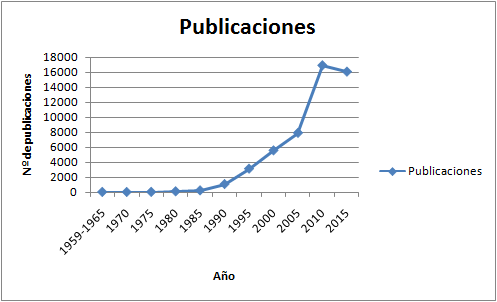
\includegraphics[width=0.9\textwidth]{./imagenes/publicaciones}
	\captionsetup{justification=centering}
	\caption{Resultados de b\'{u}squeda en el sitio web \textit{ieee explore} \cite{ieee1} con las palabras <<image segmentation>> }
	\vspace{2 mm}			
	Fuente: \cite{ieee1}
	\label{regisIEEE}
\end{figure}
 
\section{Aplicaciones}

Las aplicaciones de segmentaci\'{o}n de im\'{a}genes son muchas y muy diversas. Cualquier proceso que requiera la extracci\'{o}n de informaci\'{o}n de una imagen utilizar\'{a}, en cierta medida, una t\'{e}cnica de segmentaci\'{o}n. A continuaci\'{o}n nombraremos algunas de las aplicaciones que se han ido recopilando en la realizaci\'{o}n de esta documentaci\'{o}n, aunque el n\'{u}mero de aplicaciones totales es mucho mayor:

\begin{itemize}
	\item Localizaci\'{o}n de mol\'{e}culas en im\'{a}genes microsc\'{o}picas.
	\item Aplicaciones m\'{e}dicas.
			\begin{itemize}
				\item Localizaci\'{o}n de tumores y otras patolog\'{i}as.
			\end{itemize}
	\item Detecci\'{o}n de cuerpos para aplicaciones de seguimiento de movimientos como Kinect.
		\begin{itemize}
			\item Operaciones guiadas por ordenador.
		\end{itemize}
	\item Localizaci\'{o}n de objetos en im\'{a}genes de sat\'{e}lite.
	\item Visi\'{o}n por computador.
	\item Reconocimientos faciales.
	\item Reconocimiento de plantas
\end{itemize}